% !TEX encoding = UTF-8
% !TEX TS-program = pdflatex
% !TEX root = ../tesi.tex

%**************************************************************
\chapter{Analisi dei dati}
%\label{cap:flow engine}
%**************************************************************
\intro{Nel seguente capitolo verrà illustrata la fase di preprocessing e l'analisi grafica dei dati. }\\

%*************************************************************

\section{Preprocessing dei dati}
Dopo aver importato il dataset sul software R, il primo step da effettuare durante il prepocessing è individuare e risolvere possibili anomalie nei dati per poter poi effettuare analisi preliminari.\\
Il dataset è stato importato in modo tale che la prima riga contenga l'intestazione, mentre le restanti righe tutte le osservazioni. Il commando usato per importare il dataset è il seguente:\\

\begin{lstlisting}[language=R]
> soccer<-read.xlsx("SerieA.xlsx", 1, header=TRUE)
\end{lstlisting}
\bigskip
Il dataset non ha valori mancanti. Questo è stato possibile grazie a una buona fonte di dati che ha messo a disposizione dati quasi sempre completi; in quei rari casi di mancanza di dati sono stati reperiti manualmente da altre fonti altrettanto attendibili.\\
Sono state inoltre tolte le variabili \texttt{Date} e \texttt{Round}.\\
Il passo successivo è stato controllare se le variabili venivano interpretate con il tipo corretto. Le variabili \texttt{Team} e \texttt{Vs} vengono interpretate erroneamente come tipo \texttt{character}. Queste variabili devono essere interpretate come fattore cioè un variabile non numerica, espressa in termini verbali ad esempio una categoria; quindi ogni squadra sarà un livello del fattore. Analogamente per \texttt{AtHome} vi è un interpretazione sbagliata; ciononostante si pensi che possa essere un tipo \texttt{logical} si è preferito convertire la variabile in un fattore con due livelli. Anche la variabile \texttt{Res} è stata trasformata in un fattore con i livelli; 1 = vittoria, 0 = pareggio, -1 = sconfitta.


\section{Analisi grafica dei dati}
In questa sezione attraverso il supporto di grafici, si analizzerà graficamente i dati disponibili e le loro relazione per avere una prima visione dei dati raccolti. Si cercherà di: individuare possibili outliers o anomalie, quali distribuzioni hanno i dati ma soprattutto valutare le relazione tra covariate e variabile di risposta e tra due covariate, con lo scopo di individuare quali covariate possono essere significative per la variabile risposta e quali interazioni tra covariate emergono dall'analisi grafica.\\

Come primo passo dell'analisi, viene valutata la distribuzione delle classi della variabile risposta \texttt{Res} all'interno delle osservazioni disponibili. Tale distribuzione è mostrata nella Figura \ref{fig:res}.

\begin{figure}[htbp]
	\begin{center}
		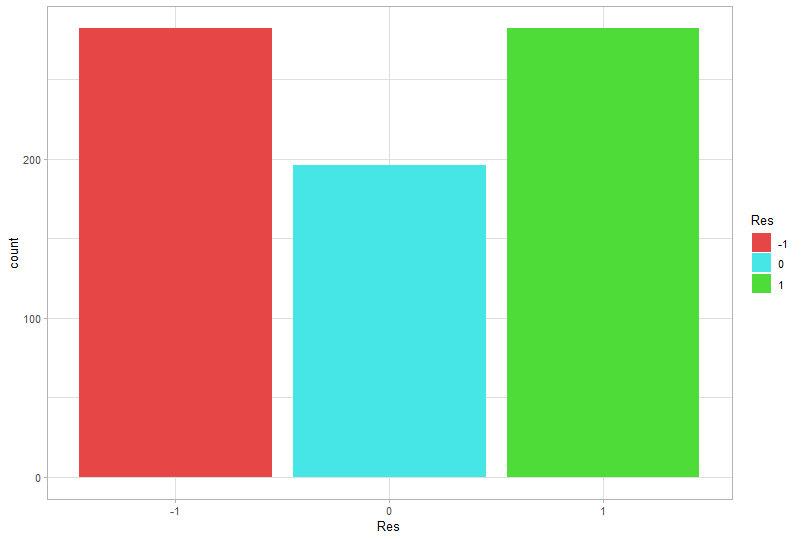
\includegraphics[scale=0.28]{barRes.png}
		\caption{Barplot della distribuzione della variabile di risposta \texttt{Res}} \label{fig:res}
	\end{center}
\end{figure}

Come si può notare le classi sembrano ben distribuite dato che abbiamo 196 pareggi e 282 vittorie e altrettante sconfitte. Si ha quindi un campione abbastanza ampio e distribuito e corretto per le nostre analisi.\\

Aumentando il livello di dettaglio è di interessante analizzare come queste classificazione sono distribuite tra le varie squadre.

\begin{figure}[htbp]
	\begin{center}
		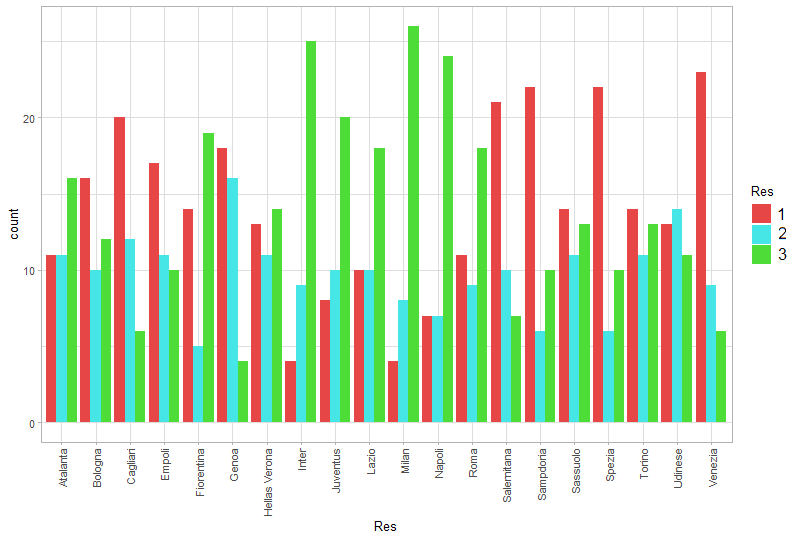
\includegraphics[height=8cm,width=15cm]{ResTeam.png}
		\caption{Barplot della distribuzione della variabile di risposta per squadra\texttt{Res}} \label{fig:team}
	\end{center}
\end{figure}

Nella Figura \ref{fig:team} si può notare come la distribuzione di vittorie, pareggi e sconfitte non è omogenea tra le squadre. Ovviamente è un risultato che ci si aspettava ma che sottolinea prima di tutto la correttezza dei dati ma soprattutto che vi è qualche elemento nascosto che ha determinato tale distribuzione.\\

\subsection{Analisi relazione tra variabile risposta e covariate}
Come secondo step si analizzerà le relazione tra variabile di risposta con alcune covariate.\\

La prima relazione che si analizza è quella con la variabile categorica \texttt{AtHome}. Nella Figura \ref{fig:AtHome} si può vedere che c'è una leggera variazione dei risultati tra la squadra che gioca in casa oppure no. Infatti c'è una leggera tendenza a favorire la vittoria per la squadra che gioca in casa piuttosto che la vittoria per la squadra fuori casa. Naturalmente non deve esserci alcuna variazione per quanto riguarda il pareggio dato che entrambe le squadre lo ottengono. Risulta perciò significativa la variabile \texttt{AtHome}.\\

\begin{figure}[htbp]
	\begin{center}
		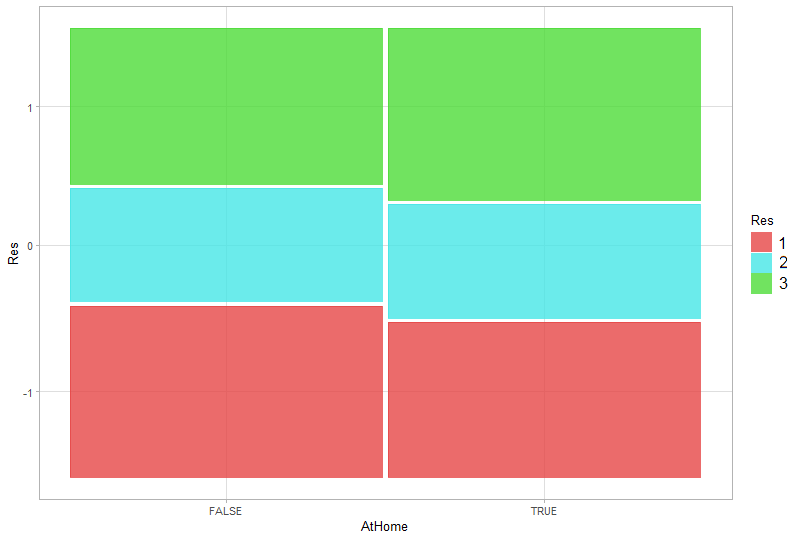
\includegraphics[scale=0.40]{AtHomeRes.png}
		\caption{Mosaicplot che mostra la distribuzione degli esiti rispetto alle partite giocate in casa e fuori casa} \label{fig:AtHome}
	\end{center}
\end{figure}

Analizzando invece la relazione tra variabile di risposta e \texttt{Poss}, dalla Figura \ref{fig:Poss} si nota che tale variabile sembra essere significativa per l'esito. Infatti vi è un relazione positiva dove, valori più alti di possesso palla sono registrati nel box della vittoria e ciò può portare a una maggiore probabilità di vittoria. Vi è una buona distribuzione dei dati, infatti le code sono simmetriche mentre vi è una variabilità quasi identica; si segnala solo che la mediana della sconfitta è più vicina al 3$^{\circ}$ quantile mentre quella della vittoria è più vicina al 1$^{\circ}$ quantile. Inoltre non vi sono presenti outliers.\\

\begin{figure}[htbp]
	\begin{center}
		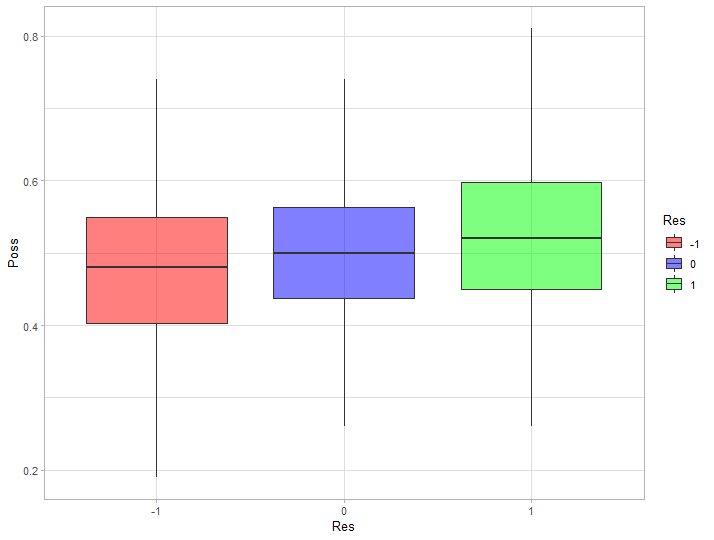
\includegraphics[scale=0.40]{Poss.png}
		\caption{Boxplot della variabile risposta e della variabile numerica \texttt{Poss} } \label{fig:Poss}
	\end{center}
\end{figure}

La Figura \ref{fig:sot} mostra come si comporta la relazione con \texttt{SoT}. Come ci si aspetta si hanno valori più alti nella vittoria e valori molto più bassi nella sconfitta, si ha una buona distribuzione dei valori nella vittoria dato che le code sono simmetriche, per le altre due classi non c'è simmetria dato che ci sono valori più bassi rispetto a valori più alti. Vi sono inoltre alcuni outliners che si discostano dalla distribuzione di tutte e tre le classi dovuti al fatto che ci sono state squadre che hanno tirato molto in porta. Le mediane dei box pareggio e vittoria non sono equidistanti dai quantili ma più vicine al 1$^{\circ}$ quantile. Il box della sconfitta ha una bassa varianza. In conclusione avere un valore alto di tiri in porta sembra essere significativo ai fini della vittoria. Si segnala inoltre che si ottengono i stessi risultati anche con \texttt{Sh} solo con valori meno alti per la vittoria rispetto a \texttt{SoT}.\\

\begin{figure}[htbp]
	\begin{center}
		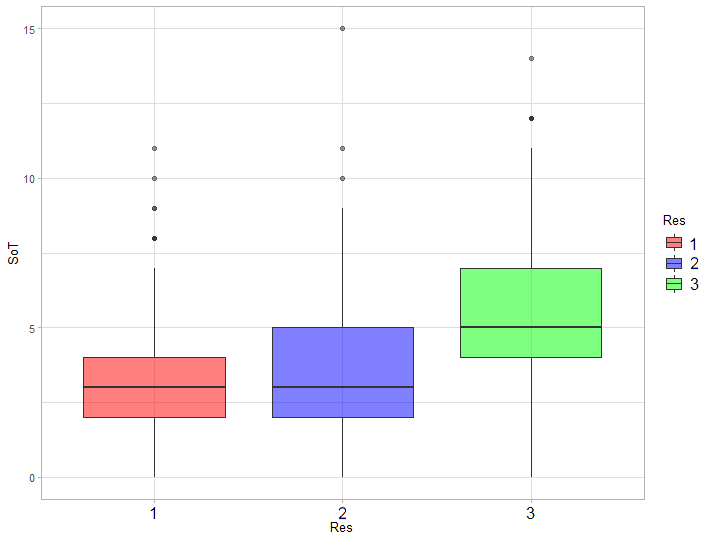
\includegraphics[scale=0.40]{SoT.png}
		\caption{Boxplot della variabile risposta e della variabile numerica \texttt{SoT} } \label{fig:sot}
	\end{center}
\end{figure}

La Figura \ref{fig:g} mostra come si comporta la relazione con \texttt{G/Sh}. Si nota che vi sono valori molto bassi ma leggermente più alti per la vittoria. La distribuzione non è buona perché le code sono asimmetriche infatti tutti i valori sono concentrati in basso e pochi verso la coda in alto, per di più c'è una bassa varianza tra i valori. Vi è la presenza di outliners dovuti a partite dove le squadre sono riuscite a ottenere il massimo da ogni tiro. I risultati mostrati nonostante la pessima distribuzione, sono comunque coerenti dato che non ci si aspetta dal rapporto tiri gol un numero alto ma comunque una tendenza che favorisca la vittoria.\\

\begin{figure}[htbp]
	\begin{center}
		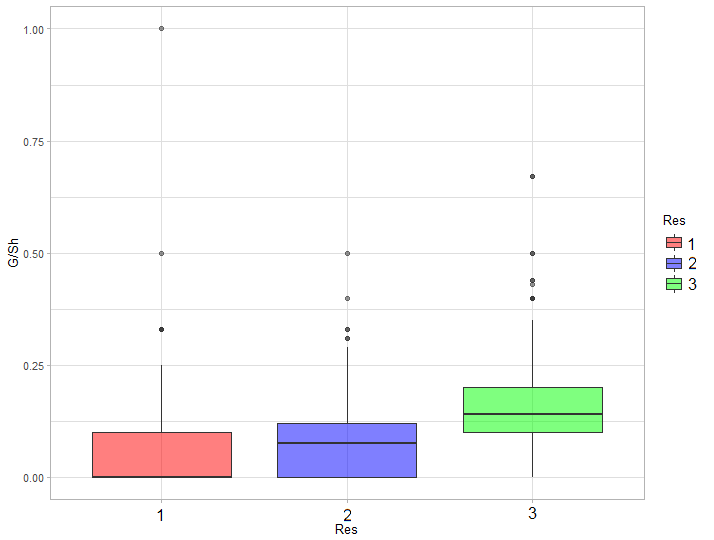
\includegraphics[scale=0.40]{g.png}
		\caption{Boxplot della variabile risposta e della variabile numerica \texttt{G/Sh} } \label{fig:g}
	\end{center}
\end{figure}

La Figura \ref{fig:saves} mostra come si comporta la relazione con \texttt{Saves}. Come si può notare sembra che tale variabile sia poco significativa ai fini del risultato. Infatti c'è poca variazione tra una classe e l'altra dato che avere un alto numero di parate non è determinante a fini del risultato.\\

\begin{figure}[htbp]
	\begin{center}
		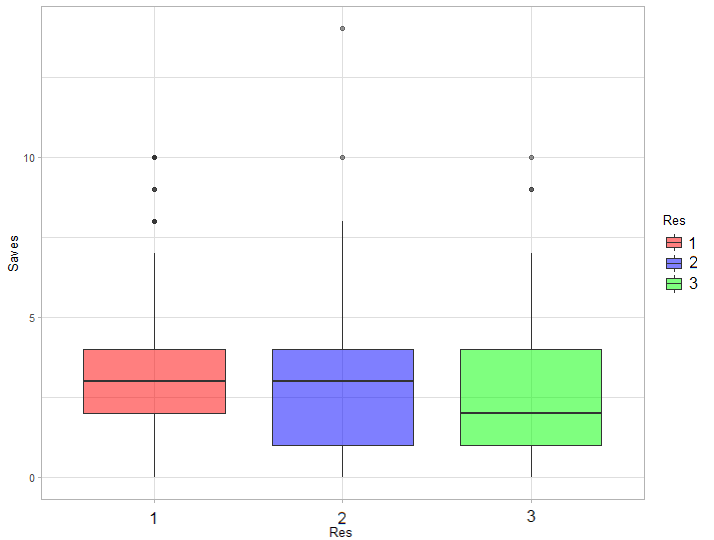
\includegraphics[scale=0.40]{saves.png}
		\caption{Boxplot della variabile risposta e della variabile numerica \texttt{Saves} } \label{fig:saves}
	\end{center}
\end{figure}

La Figura \ref{fig:pass} mostra come si comporta la relazione con \texttt{PAtt} e con \texttt{PCmp\%}. Per entrambi sembra significativo l'alto numero di passaggi tentati ma soprattutto quelli completati ai fini della vittoria. Nel primo boxplot la coda più in alto è più lunga rispetto alla coda più in basso, quindi abbiamo valori più concentrati verso il basso che verso l'alto. Sempre nel primo boxplot il box della vittoria ha una maggiore variabilità rispetto ai altri due è varia di più avendo valori più alti; sia la mediana del box vittoria e sia quello del pareggio sono più vicine al 1${^\circ}$ quantile, viceversa quella della sconfitta. I dati nel primo boxplot sembrano essere coerenti con l'esito della partita dato che maggior numero di passaggi si prova ad effettuare maggiori sono le possibilità di vittoria, occorre pero sapere quanto è precisa la squadra.\\
Nel secondo boxplot si notano valori alti e molti outliners con valori bassi dovuti al fatto che ci sono state partite dove alcune squadre sono state poco precise nei passaggi. A differenza del primo boxplot il secondo boxplot ha molti valori alti, infatti la coda più in alto e molto meno lunga rispetto alla coda più in basso e le variabilità dei box sembrano essere uguali tra di loro; anche qui le code non sono simmetriche e quindi non c'è una buona distribuzione dei dati. Sorprendentemente sembra che avere un buona precisione pero non da la sicurezza di una vittoria, inoltre l'andamento prima scende da sconfitta a pareggio e poi sale da pareggio a vittoria.\\
Per quanto riguarda le variabili delle altre tipologie di passaggi si discostano di poco dai boxplot in Figura \ref{fig:pass}

\begin{figure}[htbp]
	\begin{center}
		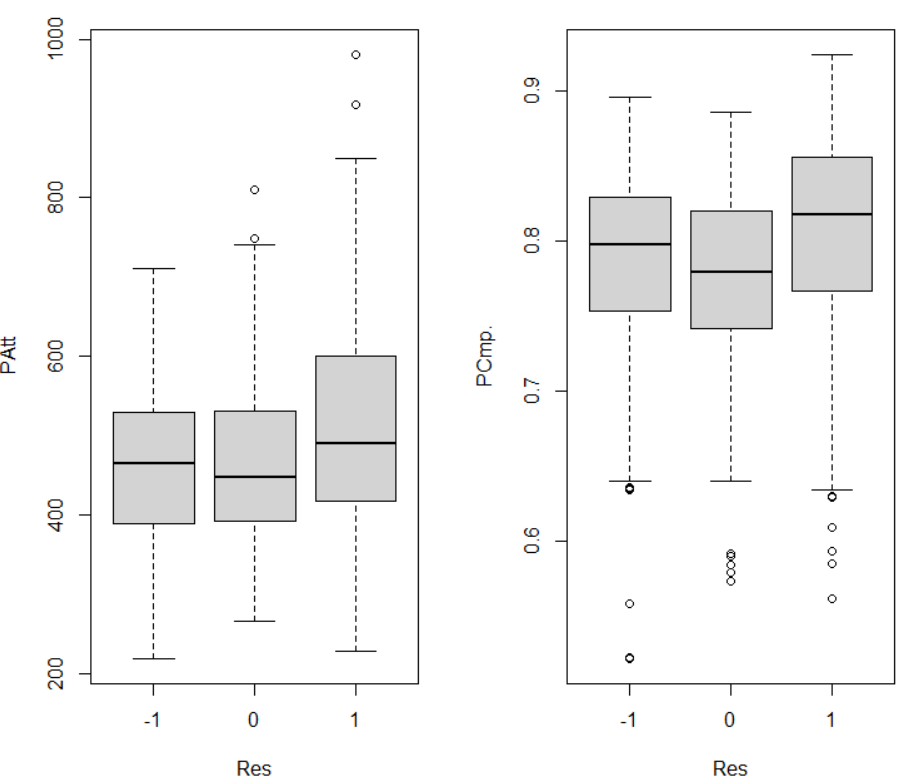
\includegraphics[scale=0.50]{pass.png}
		\caption{Boxplot della variabile risposta e della variabile numerica \texttt{PAtt} e \texttt{PCmp\%}  } \label{fig:pass}
	\end{center}
\end{figure}
\bigskip
La Figura \ref{fig:defp} mostra come si comporta la relazione con \texttt{ToDefPen}. Come si può notare questa non è per nulla significativa per la variabile risposta, infatti non c'è una minima variazione e i box hanno tutti la stessa varianza. Tale esito può essere giustificato dal fatto che le squadre cercano di rimane fuori il più possibile dalla propria area di rigore per non portare troppo vicino alla porta l'avversario. Da ciò quindi tale variabile non sarà inserita nel modello.\\

\begin{figure}[htbp]
	\begin{center}
		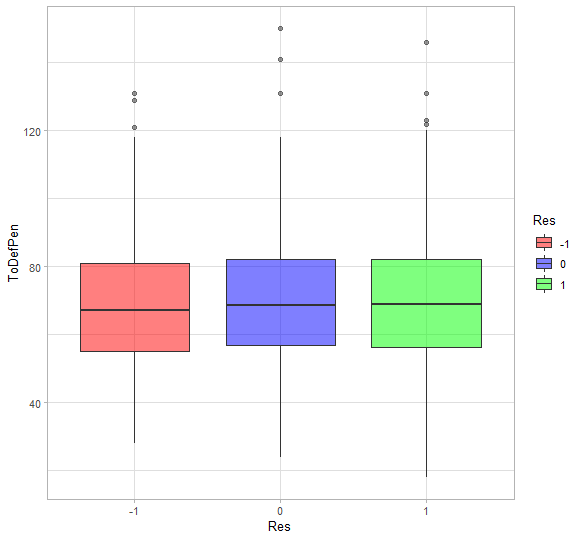
\includegraphics[scale=0.40]{def.png}
		\caption{Boxplot della variabile risposta e della variabile numerica \texttt{ToDefPen} } \label{fig:defp}
	\end{center}
\end{figure}

La Figura \ref{fig:att} mostra come si comporta la relazione con \texttt{ToAttPen}. Contrariamente quanto visto con la Figura \ref{fig:defp} qui si nota una certa variazione da una un box e l'altro, infatti vi è una tendenza positiva che porta ad aver valori più alti in caso di vittoria. Si ha una maggior varianza per quanto riguarda la vittoria rispetto ai altri due esiti e la distribuzione di tutti e tre è abbastanza bilanciata se non che la coda più bassa è leggermente meno lunga rispetto all'altra coda; la mediana invece è equilibrata. Si nota inoltre che vi sono alcuni outliners, segno che alcune squadre in qualche partita, si sono particolarmente rese note nel produrre un quantitativo di tocchi maggiore rispetto alla distribuzione, ciò pero non sembra influenzare l'esito.\\

Per quanto riguarda \texttt{ToDef3rd}, \texttt{ToMid3rd} e \texttt{ToAtt3rd}, esse si comportano come \texttt{ToAttPen}. Perciò è stato omesso il loro grafico.\\

\begin{figure}[htbp]
	\begin{center}
		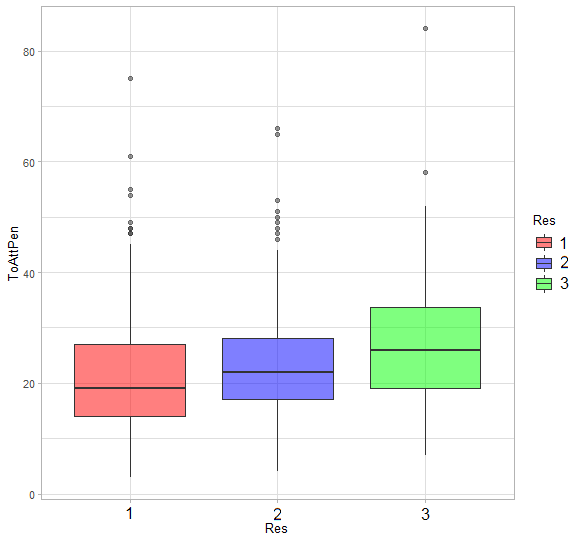
\includegraphics[scale=0.40]{att.png}
		\caption{Boxplot della variabile risposta e della variabile numerica \texttt{ToAttPen} } \label{fig:att}
	\end{center}
\end{figure}

Nella Figura \ref{fig:falli} vengono mostrati gli andamenti delle variabile dei falli, \texttt{Fls} e \texttt{Fld}. Nel boxplot a sinistra si può notare che i valori più alti sono nel box del pareggio mentre sono presenti valori più bassi nel box vittoria. Ciò fa pensare che subire molti falli può impedire la vittoria alla squadra che li subisce. Per quanto riguarda la distribuzione sembra essere buona; c'è minor varianza per quanto riguarda la sconfitta. \\

\begin{figure}[htbp]
	\begin{center}
		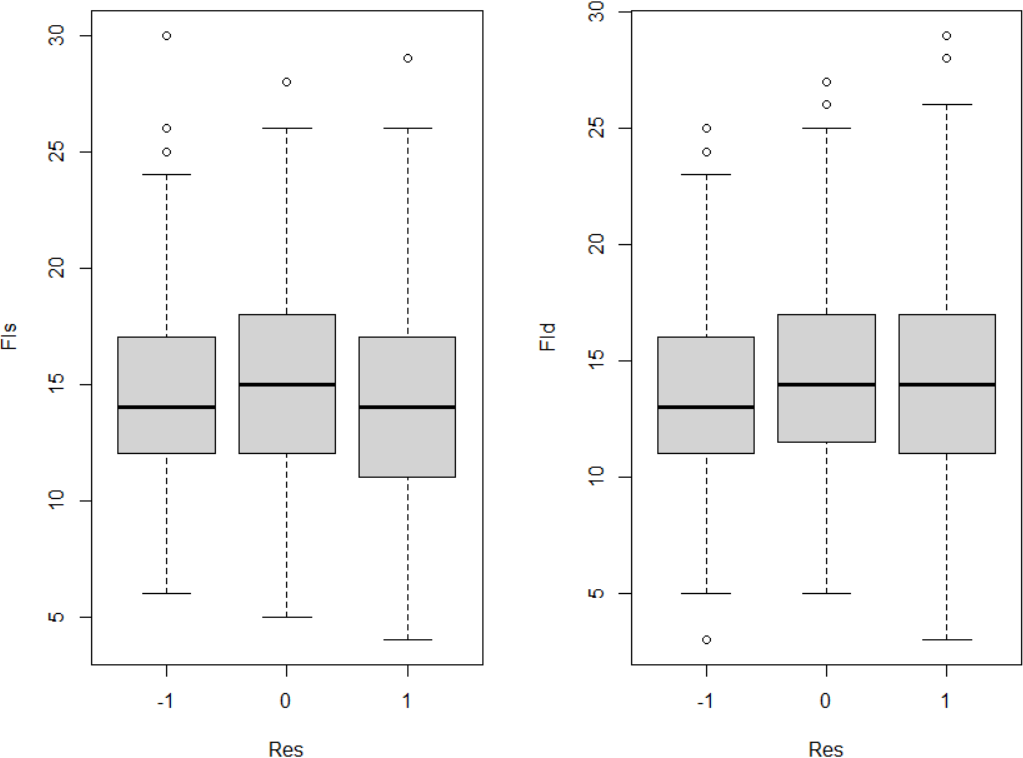
\includegraphics[scale=0.40]{falli.png}
		\caption{A sinistra il boxplot della variabile risposta e della variabile numerica \texttt{Fls} e a destra il boxplot della variabile risposta e della variabile numerica \texttt{Fld} } \label{fig:falli}
	\end{center}
\end{figure}

Nel secondo boxplot si può notare che i valori più alti sono presenti sia sul pareggio e sia sulla vittoria e sempre qui si ha una maggior distribuzione rispetto alla sconfitta. Sembra perciò che dal grafico si può intuire che se la squadra non commette dei falli allora sarà più soggetta a perdere.\\

La Figura \ref{fig:int} mostra come si comporta la relazione con \texttt{Int}. Sorprendentemente valori più alti sono registrati nella sconfitta, anche se la mediana risulta essere più vicina al 1 $^{\circ}$ quantile sottolineando che vi è un maggior numero di valori bassi piuttosto che alti. La mediana dei restanti esiti invece e ben equilibrata ma il pareggio risulta avere meno variabilità. Sembra perciò che effettuare troppi intercettazioni dei passaggi avversari contrariamente da quanto si pensi sia controproducente per la vittoria. Si segnala inoltre la presenza di alcuni outliners con valori alti di intercettazioni, che si discostano dalle distribuzioni.\\

\begin{figure}[htbp]
	\begin{center}
		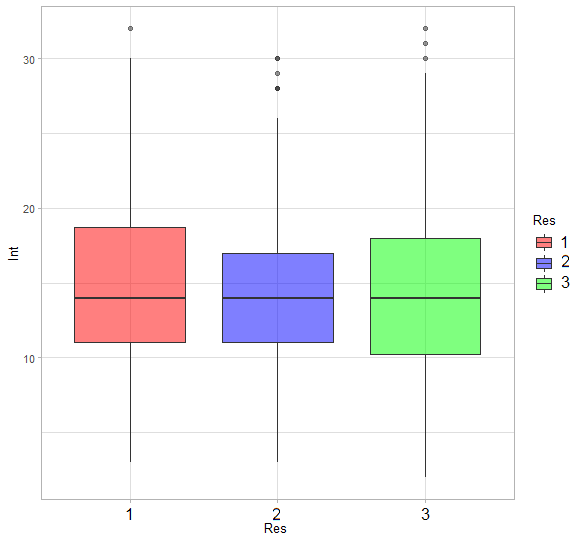
\includegraphics[scale=0.40]{int.png}
		\caption{Boxplot della variabile risposta e della variabile numerica \texttt{Int}} \label{fig:int}
	\end{center}
\end{figure}

La Figura \ref{fig:tkl} mostra come si comporta la relazione con \texttt{TklWin}. Come si può notare, vincere più contrasti possibili evita di subire una sconfitta. Infatti vi sono valori più alti in pareggio e vittoria oltre a una maggiore varianza rispetto alla sconfitta. Nello specifico pero si nota che: nella distribuzione dei valori vi sono maggior valori alti nella vittoria rispetto al pareggio, graficamente lo si vede dalla mediana che nel pareggio è più vicina al 1$^{\circ}$ quindi a valori più bassi e lo si nota anche dalla coda più bassa che è meno lunga rispetto a quella in alto; invece la mediana della vittoria risulta più vicina al 3$^{\circ}$ oltre ad avere la coda in alto più corta rispetto a quella in basso. Vi è inoltre qualche outliners con valori più alti di contrasti vinti ma sembrano non influenzare la classificazione.\\

\begin{figure}[htbp]
	\begin{center}
		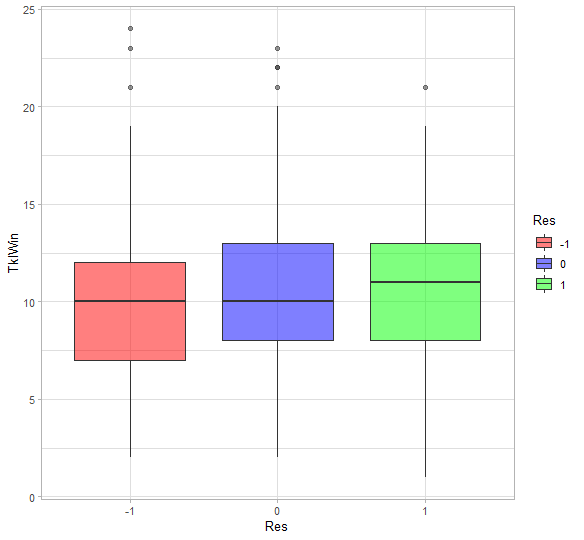
\includegraphics[scale=0.40]{tklwin.png}
		\caption{Boxplot della variabile risposta e della variabile numerica \texttt{TklWin}} \label{fig:tkl}
	\end{center}
\end{figure}

\begin{figure}[htbp]
	\begin{center}
		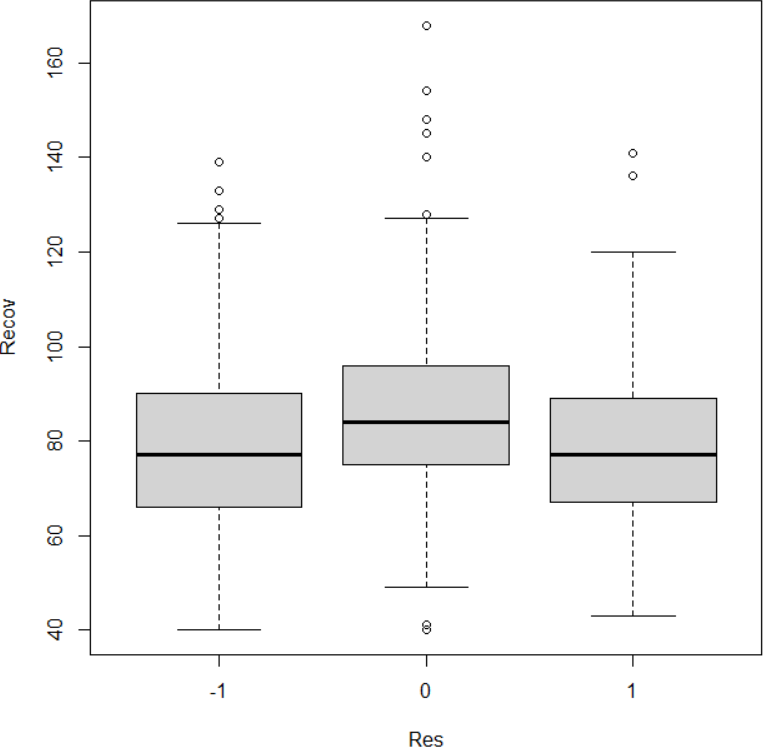
\includegraphics[scale=0.40]{recov.png}
		\caption{Boxplot della variabile risposta e della variabile numerica \texttt{Recov}} \label{fig:recov}
	\end{center}
\end{figure} 

Infine la Figura \ref{fig:recov} mostra come si comporta la relazione con \texttt{Recov}. Per entrambe le classi la distribuzione sembra più sbilanciata verso valori bassi quindi ad una loro maggior presenza, infatti entrambe le code più in basso sono più corte rispetto a quelle più in alto che sono più lunghe. Per quanto riguarda la mediana sembra equidistante dai quantili per entrambe le classi. Si nota che il pareggio presenta minor varianza rispetto alle altre due classi ma valori più alti soprattutto nei confronti della vittoria. Sembra perciò che un eccessivo numero di recuperi non porti alla vittoria. Si nota inoltre che vi sono numerosi outliners sopratutto per il pareggio.

\subsection{Analisi relazioni tra covariate} 
Per concludere l'attività di prepossening, non resta che analizzare le relazioni tra covariate in modo da individuare possibili interazioni tra di loro che possono influenzare la variabile risposta. Chiaramente dato che vi sono più di 30 variabili e dunque, un grandissimo numero di combinazioni, non si sono esaminate tutte le relazioni ma sono state selezionate solo alcune per l'analisi basandosi su teorie calcistiche esaminate durante la fase di studio del problema.\\
Di seguito si riporteranno quelle che sono state individuate come significative.\\

Sono state individuate le seguenti tre interazioni con la variabile \texttt{Sh}:
\begin{itemize}
	\item Interazione tra \texttt{Sh} e \texttt{SoT}. Chiaramente vi si può dedurre facilmente che vi possa essere una buona correlazione tra queste due variabili perché teoricamente più tiri vengono effettuati maggiori saranno i tiri in porta. \\
	Tale relazione viene anche mostrata graficamente, infatti nella Figura \ref{fig:ShSoT} si può notare che vi è un'andamento positivo tra le due variabili, al cresce di una vi è un aumento quasi lineare dell'altra.
	Come si può notare dai colori inseriti nel grafico per indicare le tre classi della variabile risposta, l'effetto combinato delle due variabili è utile a spiegare la variabile risposta dato che, valori più bassi sono quasi sempre classificati come sconfitta, un po' più alti come pareggio, mentre quelli alti sono quasi sempre classificati come vittoria.
	Molte volte i valori vengo ripetuti per molte osservazione, quindi i valori nel grafico sono disposti in colonne e non sparsi.
	\begin{figure}[htbp]
		\begin{center}
			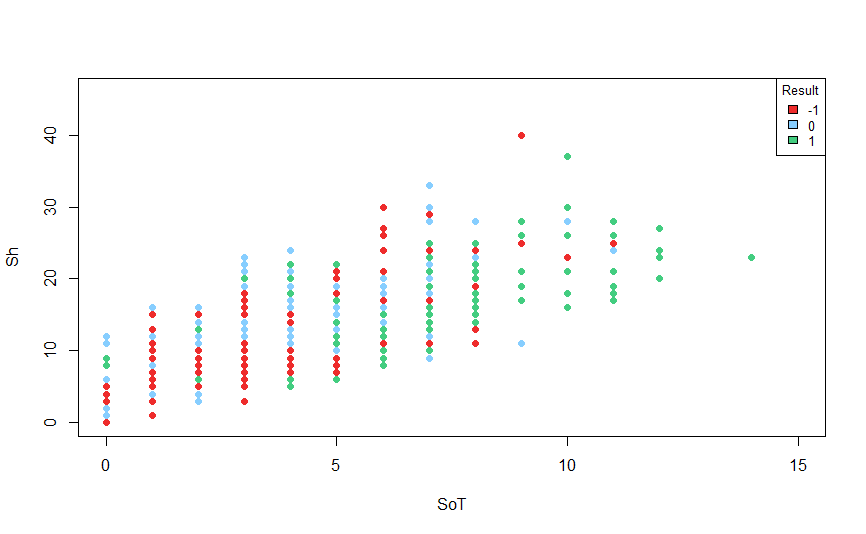
\includegraphics[scale=0.60]{sh-sot.png}
			\caption{Scatter plot tra \texttt{Sh} e \texttt{SoT}} \label{fig:ShSoT}
		\end{center}
	\end{figure} 
	\item Interazione tra \texttt{Sh} e \texttt{ToAtt3rd}. È ragionevole ipotizzare che il numero di tocchi fatti nella trequarti avversaria possano creare azioni che portano ad effettuare un tiro verso la porta avversaria; è quindi possibile che tra le due variabili vi possa esserci una relazione. L'ipotesi è avvalorata dalla Figura \ref{fig:shtreq} dove è presente una tendenza positiva quasi lineare tra le due variabili oltre a tre distribuzioni differenti dei dati in base alla loro classificazione.
	\begin{figure}[htbp]
		\begin{center}
			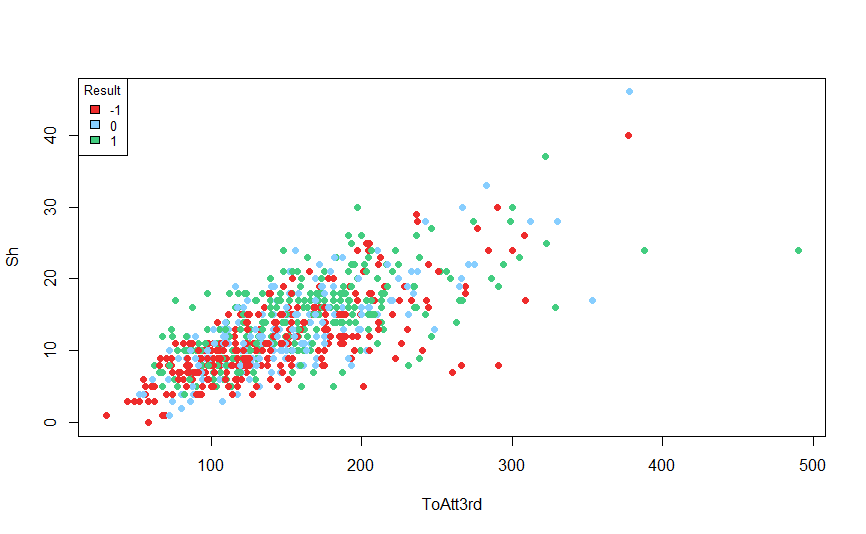
\includegraphics[scale=0.60]{sh-toatt3rd.png}
			\caption{Scatter plot tra \texttt{Sh} e \texttt{ToAtt3rd}} \label{fig:shtreq}
		\end{center}
	\end{figure}
	\item Interazione tra \texttt{Sh} e \texttt{ToAttPen}. Per la stessa ipotesi esposta nel punto precedente si è ipotizzato a tale interazione. La Figura \ref{fig:shpen} mostra che tale interazione è giustificata da una tendenza positiva nel cresce delle due variabili oltre a tre distribuzioni differenti dei dati in base alla loro classificazione. Si nota graficamente una maggior linearità rispetto alla Figura \ref{fig:shtreq}; ciò è coerente con il fatto che i tocchi vengono effettuati all'interno dell'area di rigore avversaria e quindi ad una distanza ravvicinata dalla porta, ne consegue una maggior possibilità di effettuare tiri in porta.
	\begin{figure}[htbp]
		\begin{center}
			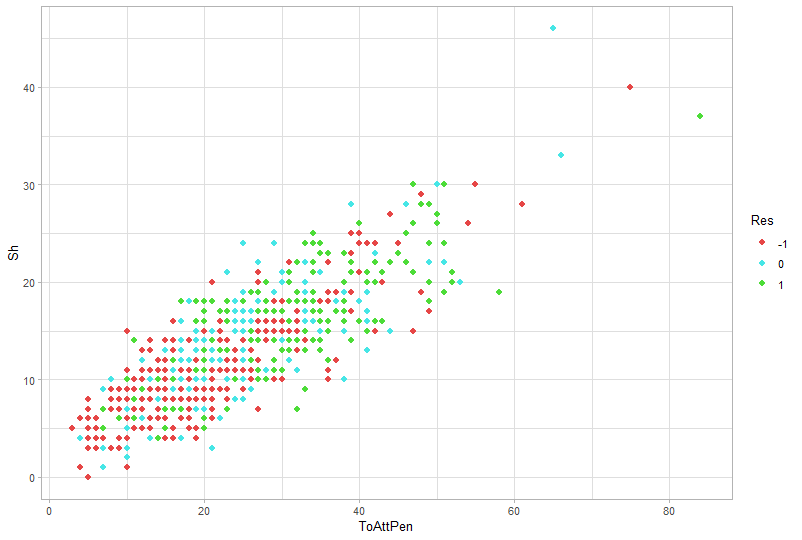
\includegraphics[scale=0.60]{sh-toattpen.png}
			\caption{Scatter plot tra \texttt{Sh} e \texttt{ToAttPen}}  \label{fig:shpen}
		\end{center}
	\end{figure}
\end{itemize}

Sono state individuate le seguenti tre interazioni con la variabile \texttt{Poss}:
\begin{itemize}
	\item Interazione tra \texttt{Poss} e \texttt{PAtt}. È ragionevole ipotizzare che il possesso della palla possa incidere su quanto una squadra tenti di effettuare passaggi, cioè da un alto possesso della palla ci si aspetta un alto numero di passaggi tentati, viceversa con un valore basso di possesso. L'ipotesi è confermata dalla Figura \ref{fig:posspatt} che mostra una relazione positiva è fortemente lineare tra le due ipotesi, oltre ad essere utili per spiegare l'andamento delle tre classi della variabile risposta.
	\begin{figure}[htbp]
		\begin{center}
			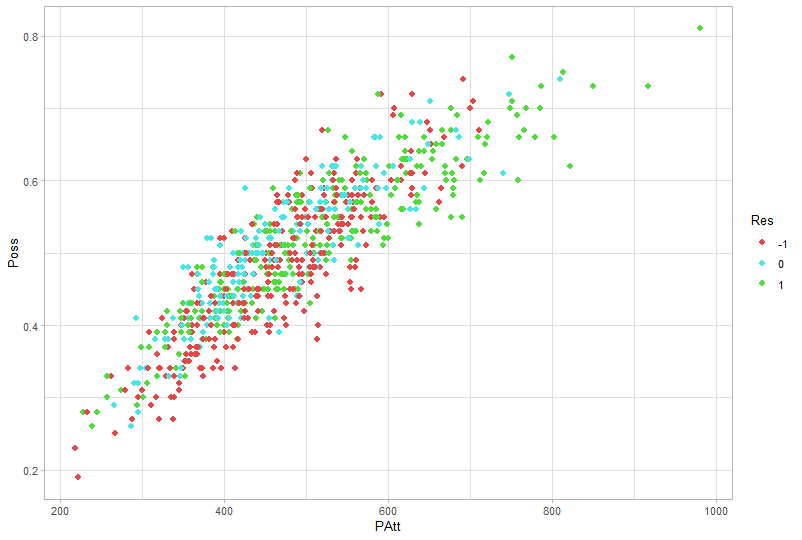
\includegraphics[scale=0.60]{poss-patt.png}
			\caption{Scatter plot tra \texttt{Poss} e \texttt{PAtt}}  \label{fig:posspatt}
		\end{center}
	\end{figure}
	\item Interazione tra \texttt{Poss} e \texttt{TotDist}. Appare naturale ipotizzare che il possesso della palla la distanza percorsa con il pallone siano in relazione tra loro. È altrettanto naturale aspettarci da un alto possesso della palla un alto numero di metri percorsi con la palla in possesso, viceversa con un valore basso di possesso. L'ipotesi è confermata dalla Figura \ref{fig:posstotdist} che mostra una relazione positiva abbastanza lineare tra le due ipotesi. Si segnala pero che dal grafico sembra che non vi sia una chiara divisione delle osservazioni in tre gruppi, tale aspetto sarà tenuto in considerazione nella modellazione.
	\begin{figure}[htbp]
		\begin{center}
			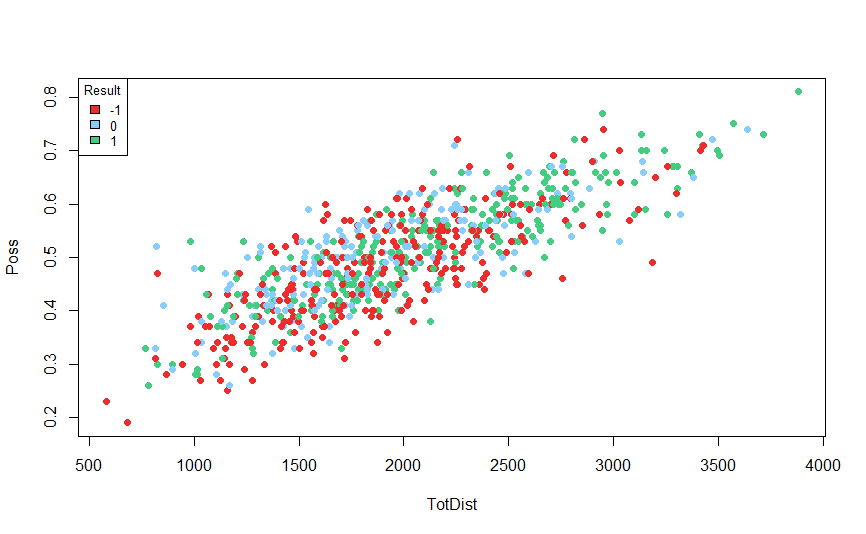
\includegraphics[scale=0.60]{poss-totdist.png}
			\caption{Scatter plot tra \texttt{Poss} e \texttt{TotDist}}  \label{fig:posstotdist}
		\end{center}
	\end{figure}
\end{itemize}
\pagebreak
Sono state individuate le seguenti tre interazioni con la variabile \texttt{TotDist}:
\begin{itemize}
	\item Interazione tra \texttt{TotDist} e \texttt{PAtt}. Dato che per poter tentare di effettuare passaggi è possibile farlo solo se ci si muove con la palla, allora è possibile ipotizzare che vi sia una relazione tra queste variabili. Dalla Figura \ref{fig:totdistpatt} si può notare che tra le due variabili vi è una forte relazione lineare e con una correlazione positiva.
	\begin{figure}[htbp]
		\begin{center}
			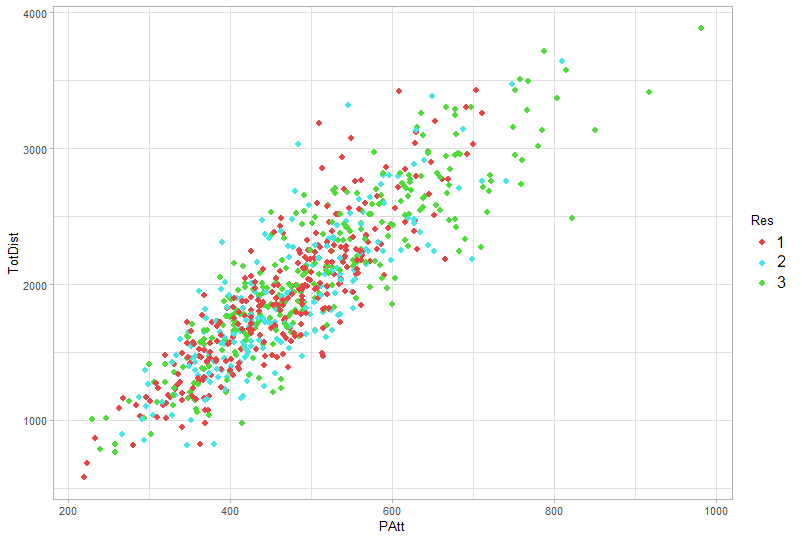
\includegraphics[scale=0.60]{TotDist-PAtt.png}
			\caption{Scatter plot tra \texttt{TotDist} e \texttt{PAtt}}  \label{fig:totdistpatt}
		\end{center}
	\end{figure}
	\item Interazione tra \texttt{TotDist} e \texttt{PCmp\%}. Dato che per poter tentare di effettuare passaggi e completarli è possibile farlo solo se ci si muove con la palla, allora è possibile ipotizzare che vi sia una relazione tra queste variabili. Dalla Figura \ref{fig:totdistpatt} si può notare che tra le due variabili vi è una relazione con correlazione positiva, con una andamento simile a una funzione esponenziale, ciò sarà tenuto conto nella modellazione per valutare se inserire oppure no una delle variabili con un grado superiore.
	\begin{figure}[htbp]
		\begin{center}
			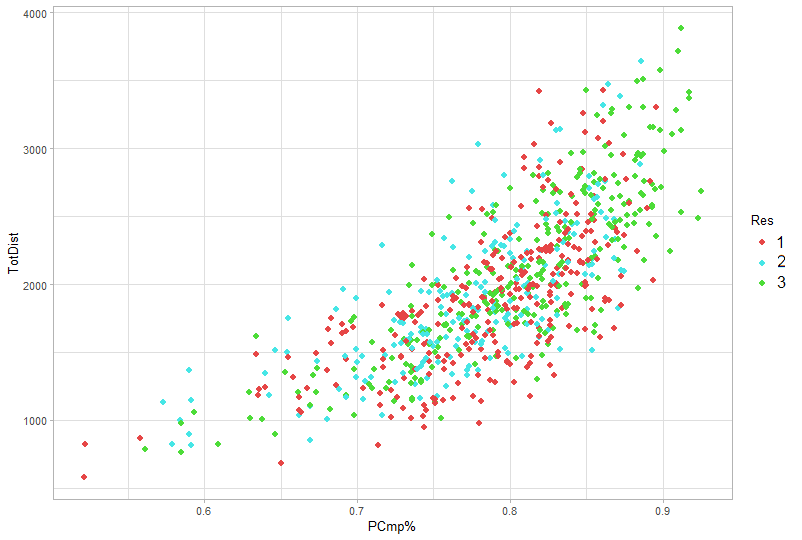
\includegraphics[scale=0.60]{TotDist-PCmp.png}
			\caption{Scatter plot tra \texttt{TotDist} e \texttt{PCmp\%}}  \label{fig:totdistpcmp}
		\end{center}
	\end{figure}
\end{itemize}

Infine sono state individuate le seguenti interazioni:
\begin{itemize}
	\item Interazione tra \texttt{ToAtt3rd} e \texttt{ToAttPen}. Dato che le due variabili si riferiscono a due zone di campo adiacenti e interessanti a fini del l'esito della partita, si ipotizza che vi sia una interazione. Nella Figura \ref{fig:toatt} si può notare un correlazione positiva molto lineare tra le due variabile che prova l'ipotesi. Si nota all'inizio che tutti i dati sono molto vicini ma che via via diventano più sparsi. Tale interazione sembra perciò utile a spiegare la variabile risposta.
	\begin{figure}[htbp]
		\begin{center}
			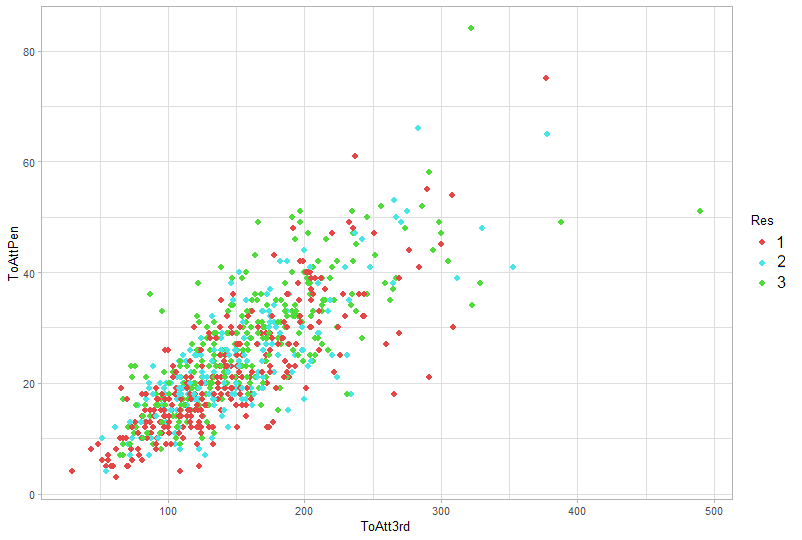
\includegraphics[scale=0.60]{ToAtt3rd-ToAttPen.png}
			\caption{Scatter plot tra \texttt{ToAtt3rd} e \texttt{ToAttPen}}  \label{fig:toatt}
		\end{center}
	\end{figure}
	\item Interazione tra \texttt{PAtt} e \texttt{PCmp\%}. Data la loro naturale correlazione si ipotizza che vi sia una interazione tra loro. Infatti tale interazione è possibile vederla nella Figura \ref{fig:pp} la quale sembra simile alla interazione \texttt{TotDist}*\texttt{PCmp\%}.
	\begin{figure}[htbp]
		\begin{center}
			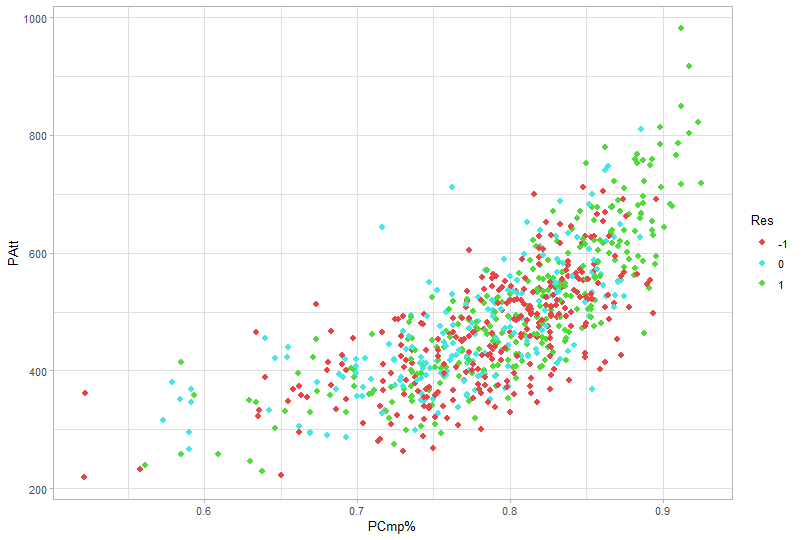
\includegraphics[scale=0.60]{PAtt-PCmp.png}
			\caption{Scatter plot tra \texttt{PAtt} e \texttt{PCmp\%}}  \label{fig:pp}
		\end{center}
	\end{figure}

\end{itemize}

\subsection{Collinearità}
Per collinearità si intende quel fenomeno per il quale se più variabili esplicative altamente correlate vengono inserite nel modello, allora la loro alta correlazione andrà a nasconde la loro associazione con la variabile risposta. La soluzione per risolvere questo problema è quella di scegliere soltanto una sola variabile della relazione da inserire nel modello.\\
Nella Figura \ref{fig:cor} viene mostrato il valore della correlazione per ogni possibile interazione tra variabile numeriche.\\
Come si può notare una maggior correlazione tra le variabile è concentra nella prima parte del triangolo. Dal grafico possiamo vedere come tutte le interazioni che sono state descritte nella sottosezione precedente abbiano un alta correlazione ma non eccessivamente alta. \\
Nella sottosezione precedente si poteva pensare di inserire interazione abbastanza naturali ad esempio: \texttt{PAtt} con \texttt{SPAtt} e con \texttt{MPAtt} e, \texttt{PCmp\%} con \texttt{MPCmp\%} e con \texttt{LPCmp\%}. Tali interazioni pero sono composte da variabili che hanno un alta correlazione tra loro, e quindi si ha il rischio di incombere in un problema di collinearità. In questa fase dell'analisi non si hanno abbastanza elementi per poter scegliere quale variabile tenere e quale no perciò tale scelta verrà rinviata alla fase di modellazione.\\
Infine si nota una buona correlazione tra \texttt{ToDefPen} e \texttt{ToDef3rd}, tale interazione non è stata inserita perché la variabile \texttt{ToDefPen} non è significativa per la variabile risposta.

\begin{figure}[htbp]
	\begin{center}
		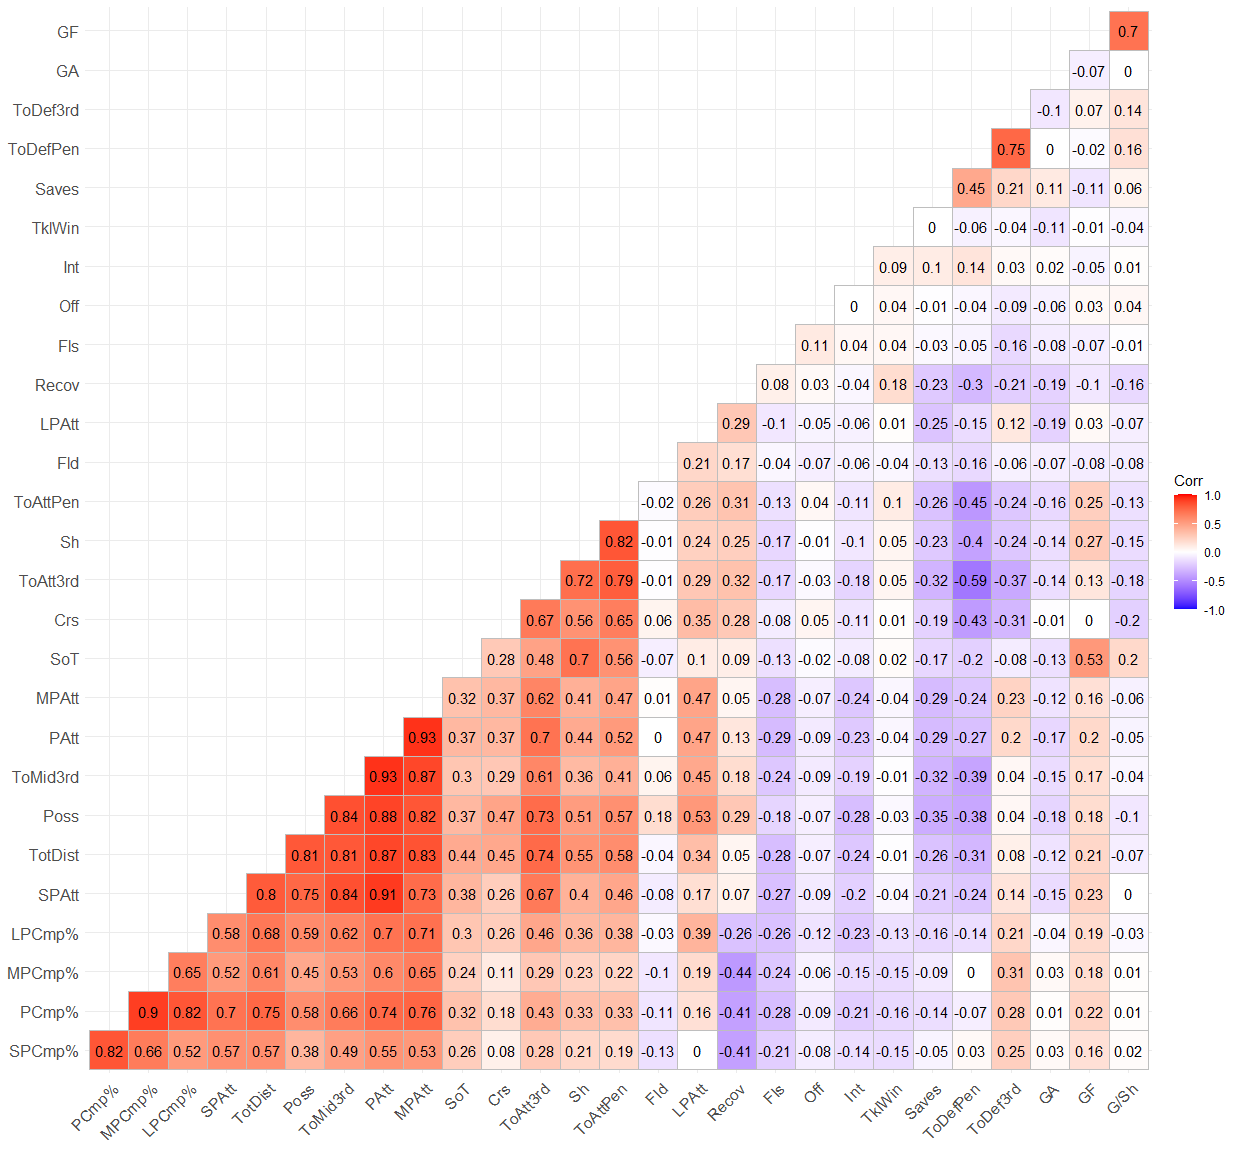
\includegraphics[scale=0.45]{Rplot.png}
		\caption{Grafico delle correlazioni di ogni coppia di variabili}  \label{fig:cor}
	\end{center}
\end{figure}

\begin{figure}[htbp]
	\begin{center}
		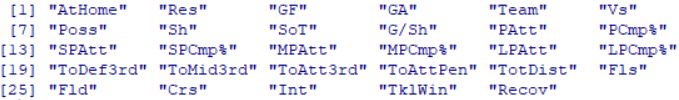
\includegraphics[scale=0.60]{cov.png}
		\caption{Grafico riassuntivo delle variabili rimaste dopo il Prepossesing}  \label{fig:cov}
	\end{center}
\end{figure}

\section{Adattamento dataset al modello}

Nelle sezioni precedenti si è descritto come si è costruito il dataset e come esso è stato strutturato. Tale struttura ha il vantaggio di rendere il dataset di facile interpretazione per un essere umano ma vi sono alcune criticità che non lo permettono di essere utilizzato correttamente all'interno del modello messo a disposizione dal pacchetto \texttt{BradleyTerry2}.\\ 
Sono state apportare alcune modifiche attraverso la scrittura di codice che andasse a modificare la struttura del dataset in modo da essere correttamente utilizzabile nel modello. \\

Innanzitutto il modello richiede per il suo funzionamento che le due variabili \texttt{Team} e \texttt{Vs} devono essere o di tipo fattore oppure un \textsf{data.frame}. Un \textsf{data.frame} è una lista di vettori, che devono avere tutti la stessa lunghezza, ma possono essere di tipo diverso: variabili nominali cioè fattori, variabili cardinali cioè vettori numerici; un \textsf{data.frame} può essere visto come una matrice ma con il tipo dei valori che può essere diverso.\\ 
Le variabili \textsf{Team} e \textsf{Vs} sono state trasformate in \texttt{data.frame} in modo da poter inserire al loro interno tutte le covariate descritte nella sezione precedente, ad esempio \textsf{Poss}, \textsf{Int} ecc.., cosi che il modello capisca quali valori sono legati alla squadra indicata in \textsf{Team} e quali in \textsf{Vs} nella stessa partita.\\

Inoltre per indicare nel modello se la squadra giocava in casa o no, i valori della variabile \texttt{AtHome} non erano accettati, si è quindi convertito il valore \texttt{TRUE} in 1 mentre FALSE in 0.



\subsection{Codice per l'adattamento del dataset}
Di seguito viene mostrato il codice applicato per adeguare il dataset con le modifiche scritte precedentemente.

\begin{lstlisting}[language=R]
PossVs <- c()
ShVs <- c()
ShTVs <- c()
G.ShVs <- c()
PAttVs <- c()
PCmp.Vs <- c()
SPAttVs <- c()
SPCmp.Vs <- c()
MPAttVs <- c()
MPCmp.Vs <- c()
LPAttVs <- c()
LPCmp.Vs <- c()
ToDef3rdVs <- c()
ToMid3rdVs <- c()
ToAtt3rdVs <- c()
ToAttPenVs <- c()
ToDistVs <- c()
FlsVs <- c()
FldVs <- c()
CrsVs <- c()
IntVs <- c()
TklWinVs <- c()
RecovVs <- c()
del <-c()
k <- 1
z <- 1

for(i in 1:nrow(soccern)){
	if(soccern$AtHome[i] == TRUE){
		for(j in 1:nrow(soccern)){
			if((soccern$Team[j] == soccern$Vs[i]) && (soccern$Team[i] == soccern$Vs[j]) && (soccern$AtHome[j] == FALSE)){
				PossVs[k] <- soccern$Poss[j]
				ShVs[k] <- soccern$Sh[j]
				ShTVs[k] <- soccern$SoT[j]
				G.ShVs[k] <- soccern$G.Sh[j]
				PAttVs[k] <- soccern$PAtt[j]
				PCmp.Vs[k] <- soccern$PCmp.[j]
				SPAttVs[k] <- soccern$SPAtt[j]
				SPCmp.Vs[k] <- soccern$SPCmp.[j]
				MPAttVs[k] <- soccern$MPAtt[j]
				MPCmp.Vs[k] <- soccern$MPCmp.[j]
				LPAttVs[k] <- soccern$LPAtt[j]
				LPCmp.Vs[k] <- soccern$LPCmp.[j]
				ToDef3rdVs[k] <- soccern$ToDef3rd[j]
				ToMid3rdVs[k] <- soccern$ToMid3rd[j]
				ToAtt3rdVs[k] <- soccern$ToAtt3rd[j]
				ToAttPenVs[k] <- soccern$ToAttPen[j]
				ToDistVs[k] <- soccern$TotDist[j]
				FlsVs[k] <- soccern$Fls[j]
				FldVs[k] <- soccern$Fld[j]
				CrsVs[k] <- soccern$Crs[j]
				IntVs[k] <- soccern$Int[j]
				TklWinVs[k] <- soccern$TklWin[j]
				RecovVs[k] <- soccern$Recov[j]
				k <- k + 1
			}      
		}
	}
	else{
		del[z] <- i
		z <- z + 1
	}
}
\end{lstlisting}
\bigskip

Con il codice precedente si ha l'obbiettivo di prendere le due righe di ogni partita e di unirle insieme formando un unica riga per ogni partita. Successivamente si elimineranno le righe delle partite giocate fuori casa (\textsf{AtHome} = FALSE) dalle squadre indicate in \textsf{Team} mentre le righe delle partite giocate in casa (\textsf{AtHome} = TRUE) dalle squadre indicate in \textsf{Team} conteranno il risultato della fusione.\\
Perciò si è creato un vettore vuoto per ogni covariata presente nel dataset, ad eccezione di \textsf{AtHome} che verrà gestita in un modo diverso. Il vettore \texttt{del} è il vettore che tiene traccia di quali righe saranno da eliminare. \texttt{k} è l'indice usato per scorre il dataset per trovare i dati dell'avversario; \texttt{z} l'indice usato per inserire un nuovo elemento nel vettore \texttt{del}.\\
Il primo ciclo \texttt{for} scorre tutto il dataset alla ricerca delle righe con i dati delle partite giocate in casa dalla squadra indicata in \texttt{Team}, infatti al suo interno il primo costrutto \texttt{if} controlla se la partita è in casa per \texttt{Team} se sì, parte un secondo ciclo \texttt{for} che anche esso scorre tutto il dataset per cercare la riga con la partita giocata della squadra indicata in \texttt{Vs}; giocata ovviamente fuori casa. Perciò all'interno del secondo ciclo \texttt{for} vi è un costrutto \texttt{if} che controlla se la j-esima riga si riferisce alla stessa partita indicata nella i-esima riga, se sì allora si salvano tutti i dati nei vettori e si incrementa l'indice \texttt{k}. Se il primo \texttt{if} da esito negativo allora si andrà a inserire l'indice dell'i-esima riga nel vettore \texttt{del} perché contiene informazioni di una partita giocata fuori casa dalla squadra indicata in \textsf{Team} e viene incrementato l'indice di uno \texttt{z}.\\

Di seguito vengono riportati i comandi fatti per applicare le modifiche al dataset.
\bigskip
\begin{lstlisting}[language=R]
> soccern3 <- soccern2[-del,]
\end{lstlisting}
\bigskip
\bigskip
Con il precedente commando si va a creare un nuovo dataset con 380 righe, eliminando tutte quelle righe con valore \texttt{FALSE} su \textsf{AtHome}. 
\bigskip
\begin{lstlisting}[language=R]
> soccern3$Team <- data.frame(team = soccern3$Team, GF = soccern3$GF, GA = soccern3$GA,  at.home = 1, Poss = soccern3$Poss, Sh = soccern3$Sh, SoT = soccern3$SoT, G.Sh = soccern3$G.Sh, PAtt = soccern3$PAtt, PCmp. = soccern3$PCmp., SPAtt = soccern3$SPAtt, SPCmp. = soccern3$SPCmp., MPAtt = soccern3$MPAtt, MPCmp. = soccern3$MPCmp., LPAtt = soccern3$LPAtt, LPCmp. = soccern3$LPCmp., ToDef3rd = soccern3$ToDef3rd, ToAtt3rd = soccern3$ToAtt3rd, ToAttPen = soccern3$ToAttPen, TotDist = soccern3$TotDist, Fls = soccern3$Fls, Fld = soccern3$Fld, Crs = soccern3$Crs, Int = soccern3$Int, TklWin = soccern3$TklWin, Recov = soccern3$Recov)
	
\end{lstlisting}

\bigskip
Con il precedente commando si va a modificare \textsf{Team} rendendolo un \texttt{data.frame}, andando a inserire i dati della riga relativi alla squadra che gioca in casa. Si inserisce come chiave \texttt{team = soccern3\$Team} e si indica che la partita è in casa per la squadra di riferimento con \texttt{at.home = 1}.
\bigskip
\bigskip
\begin{lstlisting}[language=R]
> soccern3$Vs <- data.frame(team = soccern3$Vs, GF = GFVs, GA = GAVs, at.home = 0, Poss = PossVs, Sh = ShVs, SoT = ShTVs, G.Sh = G.ShVs, PAtt = PAttVs, PCmp. = PCmp.Vs, SPAtt = SPAttVs, SPCmp. = SPCmp.Vs, MPAtt = MPAttVs, MPCmp. = MPCmp.Vs, LPAtt = LPAttVs, LPCmp. = LPCmp.Vs, ToDef3rd = ToDef3rdVs, ToAtt3rd = ToAtt3rdVs, ToAttPen = ToAttPenVs, TotDist = ToDistVs, Fls = FlsVs, Fld = FldVs, Crs = CrsVs, Int = IntVs, TklWin = TklWinVs, Recov = RecovVs)
	
\end{lstlisting}
\bigskip
Con il precedente commando si va a modificare \textsf{Vs} rendendolo un \texttt{data.frame}, andando a inserire i dati della riga relativi alla squadra che gioca fuori casa. Si inserisce come chiave \texttt{team = soccern3\$Vs} e si indica che la partita è fuori casa per la squadra \texttt{Vs} con \texttt{at.home = 0}.\\ Per quanto riguarda il resto dei dati vengo riportati attraverso l'inserimento dei vettori costruiti e riempiti precedentemente.\\
